\documentclass[tikz,border=6pt]{standalone}
\usepackage[T1]{fontenc}
\usepackage{lmodern}
\usepackage{amsmath}
\usetikzlibrary{positioning,arrows.meta,fit,calc}
% Design of koblitz-n83-stacked-20261016 (frozen protocol.json). Not a result.
\begin{document}
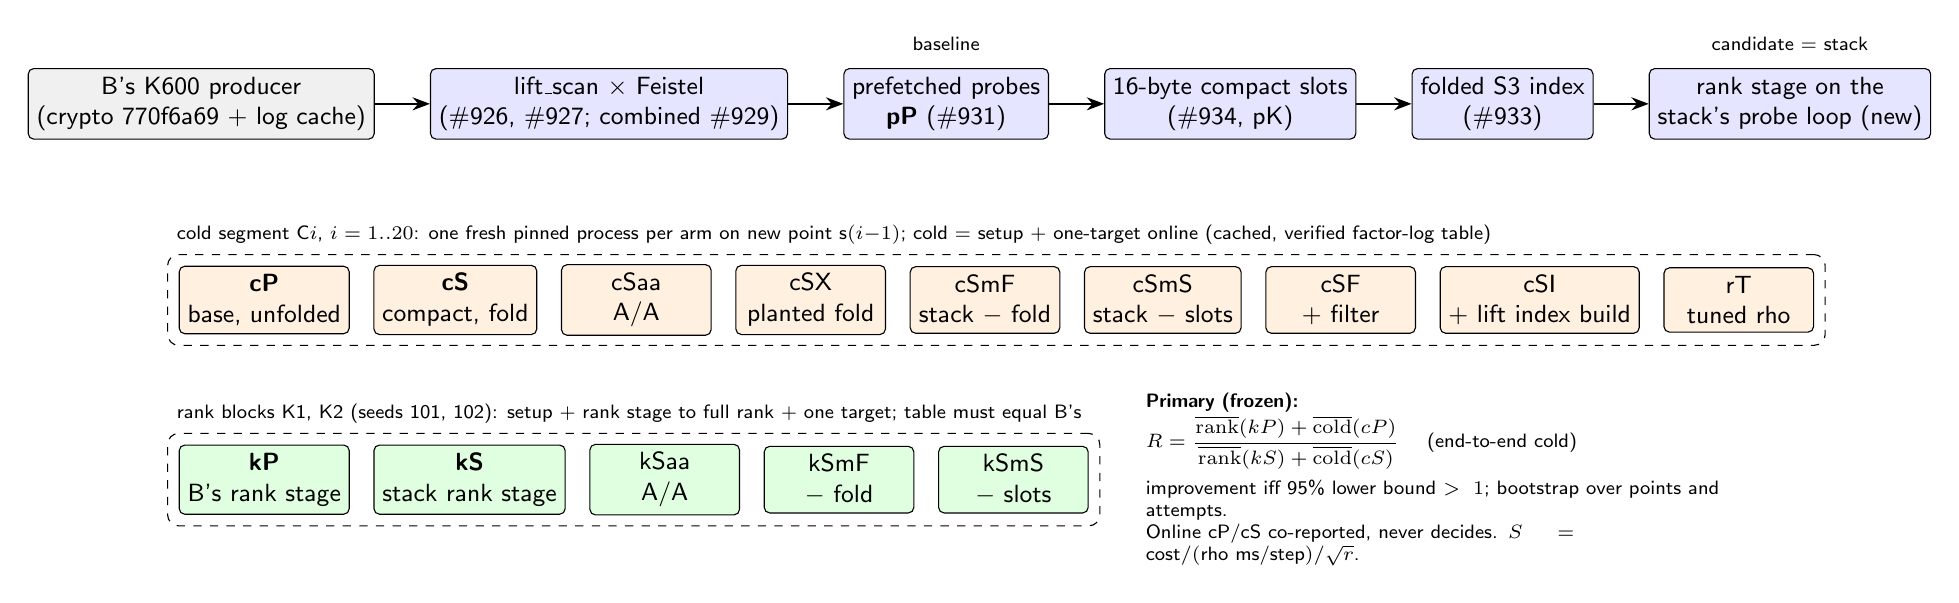
\begin{tikzpicture}[
  font=\sffamily\small,
  box/.style={draw, rounded corners=2pt, align=center, minimum height=8mm, inner sep=3pt},
  base/.style={box, fill=gray!12},
  add/.style={box, fill=blue!10},
  arm/.style={box, fill=orange!12, minimum width=19mm},
  rank/.style={box, fill=green!12, minimum width=19mm},
  arr/.style={-{Stealth[length=2.2mm]}, thick},
  note/.style={align=left, font=\sffamily\scriptsize}
]
% Stack lineage
\node[base] (b) {B's K600 producer\\(crypto 770f6a69 + log cache)};
\node[add, right=7mm of b] (c) {lift\_scan $\times$ Feistel\\(\#926, \#927; combined \#929)};
\node[add, right=7mm of c] (p) {prefetched probes\\\textbf{pP} (\#931)};
\node[add, right=7mm of p] (k) {16-byte compact slots\\(\#934, pK)};
\node[add, right=7mm of k] (f) {folded S3 index\\(\#933)};
\node[add, right=7mm of f] (r) {rank stage on the\\stack's probe loop (new)};
\draw[arr] (b) -- (c); \draw[arr] (c) -- (p); \draw[arr] (p) -- (k); \draw[arr] (k) -- (f); \draw[arr] (f) -- (r);
\node[note, above=1mm of p] {baseline};
\node[note, above=1mm of r] {candidate = stack};

% Cold arms
\node[arm, below=16mm of b, xshift=8mm] (cP) {\textbf{cP}\\base, unfolded};
\node[arm, right=3mm of cP] (cS) {\textbf{cS}\\compact, fold};
\node[arm, right=3mm of cS] (cSaa) {cSaa\\A/A};
\node[arm, right=3mm of cSaa] (cSX) {cSX\\planted fold};
\node[arm, right=3mm of cSX] (cSmF) {cSmF\\stack $-$ fold};
\node[arm, right=3mm of cSmF] (cSmS) {cSmS\\stack $-$ slots};
\node[arm, right=3mm of cSmS] (cSF) {cSF\\+ filter};
\node[arm, right=3mm of cSF] (cSI) {cSI\\+ lift index build};
\node[arm, right=3mm of cSI] (rT) {rT\\tuned rho};
\node[draw, dashed, rounded corners, fit=(cP) (rT), inner sep=4pt, label={[note, anchor=south west]north west:{cold segment C$i$, $i=1..20$: one fresh pinned process per arm on new point s$(i{-}1)$; cold = setup + one-target online (cached, verified factor-log table)}}] (cold) {};

% Rank arms
\node[rank, below=14mm of cP] (kP) {\textbf{kP}\\B's rank stage};
\node[rank, right=3mm of kP] (kS) {\textbf{kS}\\stack rank stage};
\node[rank, right=3mm of kS] (kSaa) {kSaa\\A/A};
\node[rank, right=3mm of kSaa] (kSmF) {kSmF\\$-$ fold};
\node[rank, right=3mm of kSmF] (kSmS) {kSmS\\$-$ slots};
\node[draw, dashed, rounded corners, fit=(kP) (kSmS), inner sep=4pt, label={[note, anchor=south west]north west:{rank blocks K1, K2 (seeds 101, 102): setup + rank stage to full rank + one target; table must equal B's}}] (rk) {};

\node[note, right=6mm of kSmS, text width=78mm] (eq) {\textbf{Primary (frozen):}\\
$R = \dfrac{\overline{\mathrm{rank}}(kP) + \overline{\mathrm{cold}}(cP)}{\overline{\mathrm{rank}}(kS) + \overline{\mathrm{cold}}(cS)}$ \quad (end-to-end cold)\\[1mm]
improvement iff 95\% lower bound $>1$; bootstrap over points and attempts.\\
Online cP/cS co-reported, never decides. $S = $ cost$/(\text{rho ms/step})/\sqrt{r}$.};
\end{tikzpicture}
\end{document}
